
\documentclass[a4paper,12pt,portuges]{article}
\usepackage{babel}
\usepackage[utf8]{inputenc}
\usepackage{graphicx}

\title {Relatório LI - \textit{LightBot} em \textit{Haskell}}
\author{Rogério Moreira / Samuel Ferreira}
\date {\today}

\begin {document}
\maketitle

\section {Introdução ao Projeto}

Este projeto foi desenvolvido no âmbito da disciplina de Laboratórios de Informática I da Licenciatura em Engenharia Informática na Universidade do Minho. O trabalho foi inicialmente dividido em 2 fases, uma 1º Fase que decorreu até ao dia 30 de Novembro que compreendia os três primeiros problemas e uma 2º Fase que decorreu até ao dia 5 de Janeiro que compreendia os dois últimos problemas. Todo o projeto foi desenvolvido com recurso à linguagem funcional \textit{Haskell}.\\
O projeto consiste no desenvolvimento de um conhecido jogo, que para além de ter uma componente didática ajuda também crianças a aprender as componentes básicas da programação. No \textit{Lightbot} o objetivo é controlar um Robot por intermédio de cinco comandos básicos: Avançar, Saltar, Direita, Esquerda e Ligar Lâmpada, o objetivo final do jogo é ligar todas as lâmpadas disponíveis no tabuleiro.

\section {Desenvolvimento do Projeto}

\subsection {Problema A}

O problema A consistia em validar se um input fornecido cumpria os requisitos de um tabuleiro, posição inicial e comandos válidos. O programa desenvolvido imprime dois tipos de resultado conforme o input seja ou não válido:\\

\begin{description}
\item[OK] - Se o formato do input estiver totalmente correto.\\
\item[num]- Se a linha num é a linha onde se encontra o primeiro erro.
\end{description}
\\
Do nosso ponto de vista, este foi o problema mais abstrato uma vez que não só serviu para nos ambientar com todo o sistema como a validação compreendia uma grande variedade de testes.

Em primeiro lugar definimos o que seria um input válido e todos os testes que seriam necessários:\\

\begin{description}
\item[Tabuleiro Válido] - O tabuleiro ter apenas letras maiúsculas ou minúsculas.\\
\item[Comprimento do Tabuleiro]- É necessário que todas as linhas do tabuleiro tenham o mesmo comprimento.\\
\item[Posição Inicial]- A posição inicial deve ser constituída apenas por dois números e uma orientação separados por espaços.\\
\item[Orientação] - A orientação, parte constituinte da posição inicial, deve ser um dos pontos cardeais, ou seja: N (Norte), S (Sul), O (Oeste) ou E (Este).\\
\item[Posição Inicial no Tabuleiro] - Validação se a posição inicial dada está ou não dentro do tabuleiro dado.\\
\item[Comandos] - A validação dos comandos correspondia apenas à validação das letras, tendo estas que ser maiúsculas e ser uma das opções: A (Avançar), S (Saltar), L (Acender Luz), D (Rodar à direita) e E (Rodar à esquerda).\\
\end{description}
\\
No decorrer da execução da tarefa pensamos em mais alguns testes como por exemplo a validação se todas as lâmpadas eram acessíveis contudo e depois de executados estes testes a pontuação no \textit{Mooshak} diminuía, posto isto decidimos retirar os testes.
\\
Das funções desta tarefa podemos referir três principais. São estas funções que selecionam do input aquilo que é suposto ser o tabuleiro, a posição inicial e os comandos e que vão permitir correr todos os outros testes nas respetivas partes do input inicial.\\

    
\textbf{Seleção do Tabuleiro}
\begin{verbatim}
selTab :: [String] -> [String]
selTab [] = []
selTab inp = takeWhile (notElem ' ') inp
\end{verbatim}

\\

Esta função corre todo o input até encontrar um espaço. Quando encontrar o espaço em branco a função devolve tudo o que está para trás, permitindo assim selecionar o tabuleiro de uma maneira eficaz e que permite em input's não válidos selecionar corretamente o tabuleiro. A função \textit{selTab} é a função mais importante das três uma vez que as outras recorrem a esta para selecionar tanto a posição inicial como os comandos.\\

\textbf{Seleção da Posição Inicial}
\begin{verbatim}
selPos :: [String] -> String
selPos [] = []
selPos inp =  inp !! (length (selTab inp))
\end{verbatim}
\\
Esta função recorre ao selTab e retira o elemento do input correspondente ao comprimento do selTab do input. Uma vez que a função  \textit{(!!)} do \textit{Haskell} começa a sua contagem a partir do 0, ou seja, o primeiro elemento do input é o elemento 0.\\

\textbf{Seleção dos Comandos}
\begin{verbatim}
selCom :: [String] -> String
selCom [] = []
selCom inp = inp !! (length (selTab inp) +1)
\end{verbatim}
\\

Esta função recorre mais uma vez ao \textit{selTab} e retira o suposto último elemento da lista. Como não sabemos se o input é válido, ou seja, não sabemos se o input termina com os comandos do Robot então temos que o selecionar a partir do \textit{selTab}. Os comandos correspondem ao comprimento do \textit{selTab} somado com um, porque, como já foi explicado anteriormente, a função \textit{(!!)} começa a sua contagem em 0.\\

Esta tarefa foi concluída com a pontuação máxima dos testes realizados no \textit{Mooshak}, 15 pontos.\\

\subsection {Problema B}

O problema B consistia em implementar um programa que determinasse qual a posição do robot após a execução do primeiro comando fornecido. Existem, tal como no Problema A dois outputs:\\

\begin{description}
\item[ERRO] - Se o comando não for possível (ex: acender uma lâmpada numa posição que não tem lâmpada ou avançar para uma posição que não pertence ao tabuleiro).\\
\item[xcoord ycoord orient] - Caso o comando seja aplicável (onde xcoord, ycoord e orient denotam respetivamente as coordenadas x e y do robot, e orient a sua orientação após a execução do comando).
\end{description}
\\

Este problema sintetiza-se numa função, que calcula a posição após a execução do primeiro comando.

\begin{verbatim}
tarefa :: [String] -> [String]
tarefa [] = []
tarefa input = [linha]
where linha | primcomando == 'E' = convertToString (esquerda posicao)
| primcomando == 'D' = convertToString (direita posicao)
| primcomando == 'L' && isUpper (indice posicao tabuleiro) = convertToString posicao
| primcomando == 'A' && testacoord tabuleiro (proximaPos posicao)
      && altura (proximaPos posicao) tabuleiro == altura posicao tabuleiro
      = convertToString (proximaPos posicao)
| primcomando == 'S' && testacoord tabuleiro (proximaPos posicao)
      = if altura (proximaPos posicao) tabuleiro < altura posicao tabuleiro 
|| altura (proximaPos posicao) tabuleiro == (altura posicao tabuleiro) +1
then convertToString (proximaPos posicao)
else "ERRO"
| otherwise = "ERRO"
\end{verbatim}

Quando começamos a pensar neste problema pensamos logo numa função recursiva que percorre uma série de opções até encontrar a opção correspondente ao primeiro comando. Contudo, tivemos também que ter uma série de cuidados na execução dos comandos:\\
\begin{description}
\item[Comando L (Ligar Lâmpada)] - No comando L temos que ter em atenção que a posição onde estamos a tentar ligar a lâmpada corresponde realmente a uma lâmpada do tabuleiro.\\
\item[Comando A (Avançar)]- No comando A temos que ter em atenção duas coisas, a primeira é que a coordenada depois de avançar está dentro do tabuleiro e a segunda é que a próxima posição tem o mesmo nível, ou seja, que não é preciso executar antes o comando S (Saltar).\\
\item[Comando S (Saltar)] - No comando S temos que ter em atenção que o nível da coordenada é apenas uma vez superior ao nível da coordenada atual, assim como que essa coordenada está dentro do tabuleiro.\\
\end{description}

Esta tarefa foi concluída com a pontuação máxima dos testes realizados no \textit{Mooshak}, 15 pontos.\\

\subsection {Problema C}


O problema C, último problema da 1º Fase do Projeto de Laboratórios de Informática I consistia em executar a sequência total dos comandos no Robot. Tendo em conta os seguintes aspetos:\\

\begin{itemize}
\item Os comandos tinham que ser executados em sequência. \\
\item Os comandos que não podem ser aplicados deixariam o Robot na mesma posição.\\
\item Sempre que um comando L for executado com sucesso deveria ser impressa uma linha contendo as cordenadas x e y da posição onde o robot se encontra.
\end{itemize}
\\

Pensamos nesta tarefa como uma recursividade da tarefa B, uma vez que já na tarefa B tínhamos realizado uma tarefa que executava o primeiro comando. Contudo e como descrito mais à frente esta não foi a melhor estratégia já que se revelaria bastante lenta na execução de tabuleiros com grandes dimensões.\\
Este problema tinha dois tipos de outputs:\\  

\begin{description}
\item[FIM] - Se todas as lâmpadas do tabuleiro se encontrarem ligadas depois de executados todos os comandos, seguido do número total de comandos executados com sucesso.\\
\item [INCOMPLETO] - Se a sequência de comandos terminar sem que todas as lâmpadas tenham sido ligadas.
\end{description}
\\
De referir duas funções usadas na resolução deste problema:\\

\textbf{Função que devolve a lista de lâmpadas de um tabuleiro.} \\
\begin{verbatim}
stlampadas :: [String] -> Int -> [String]
stlampadas [] _ = []
stlampadas (h : t) n = (aux h (length (h:t) -1) 0) ++ (stlampadas t (n-1))
 where aux [] _ _ = []
aux (x:xs) l c | isUpper x = (show c ++ " " ++ show l) : aux xs l (c+1) 
| otherwise = aux xs l (c+1)
\end{verbatim}
\\
\textbf{Função que executa a recursividade sob a lista de comandos.} \\
\begin{verbatim}
executa :: [String] -> String -> String -> [String] ->Int -> [String]
executa _ _ [] l n | l == [] = ["FIM " ++ show n]
                   | otherwise = ["INCOMPLETO"]
executa t p c l n | l == [] = ["FIM " ++ show n]
                  | tarefaB set == ["ERRO"] = executa t p (tail c) l n 
                  | tarefaB set == [p] && (head c) == 'L' = [take (length p -2) p] ++ executa t p (tail c) (upLight (take (length p -2) p) l) (n+1)
                  | otherwise = executa t (head (tarefaB set)) (tail c) l (n+1)
                    where set = (t++[p]++[c])
\end{verbatim}


A estratégia que adotamos (recursividade sob os comandos) embora funcionasse não se revelou a melhor para tabuleiros de grandes dimensões, uma vez que demora bastante tempo a executar. Posto isto, em alguns testes disponibilizados no \textit{Mooshak} com tabuleiros de grandes dimensões o programa não executou a totalidade do input resultando no erro \textit{Time Limit Exceed}, já que o tempo dado para a execução foi inferior aquele que a função demorava para realmente executar o teste. Esta tarefa foi assim concluída com a pontuação 17 pontos em 20 no \textit{Mooshak}.\\

\subsection {Problema D}

O problema E era, por ventura, o problema com a resolução mais difícil não só porque existiram diversas maneiras de o resolver mas também pelo facto do número de casos possíveis ser bastante elevado. Este problema consistia em calcular todos os comandos necessários para completar um tabuleiro, ou seja, ligar todas as lâmpadas. O seu output era único, uma lista com todos os comandos necessários. Caso o tabuleiro não tivesse lâmpadas não existiam comandos a executar para o completar, estaria logo à partida completo.
\\
Quando começamos a pensar sobre o problema colocamos duas opções para o resolver:

\paragraph {Opção 1 - Árvores Binárias}
\\
Inicialmente pensámos em resolver o problema recorrendo a árvores binárias. Pensámos em gerar com o programa uma árvores binária com todos os caminhos possíveis dependendo das lâmpadas a que teríamos que aceder. Posto isto, seria muito mais fácil calcular o caminho mais curto para cada lâmpada, contudo colocaram-se dois problemas a esta opção. Por um lado o programa seria mais eficiente mas teríamos um problema em tabuleiros mais complexos umas vez que há a possibilidade de uma lâmpada não ser acessível a partir da posição mas tornar-se acessível depois de acendida a próxima lâmpada da árvore binária. Outro dos problemas prendia-se com o facto de o programa não ser rápido o suficiente e tornar-se ineficiente em tabuleiros de grandes dimensões.

\paragraph {Opção 2 - Listas}
\\
Chegamos então à conclusão que teríamos que usar listas normais para resolver o problema. Começamos então por reaproveitar uma função já definida no Problema D, função essa que gera a lista de lâmpadas que têm que ser acendidas para completar o tabuleiro.

\\

Este problema tinha apenas um tipo de output embora este possa variar consoante as estratégias usadas para resolver o problema. O output deve ser uma lista com todos os comandos necessários para resolver o tabuleiro do input.

\\

Uma função a referir:
\textbf{Função que percorre todas as luzes e as tentar acender, retornando os comandos.} \\
\begin{verbatim}
luzes :: [Pos] -> Pos -> Orient -> Tab -> [Cmd]
luzes [] _ _ _ = []
luzes ((x,y):[]) (a,b) orient tab | snd (move (a,b) (x,y) orient tab []) == 'I' = []
                                  | otherwise= cmd ++ "L" 
                                  where cmd = fst (move (a,b) (x,y) orient tab []) 
                       
luzes l (a,b) orient tab | elem (a,b) l = "L"++ luzes (delete (a,b) l) (a,b) orient tab
                         | snd (move (a,b) (x,y) orient tab []) == 'I' 
                         = luzes (xys++[(x,y)]) (a,b) orient tab
                         | otherwise = cmd ++ "L" ++ luzes xys (x,y) o tab
                          where (x,y)= head l
                                xys = tail l
                                (cmd,o) = (move (a,b) (x,y) orient tab [])
\end{verbatim}


\\

Apesar da resolução do problema funcionar em bastantes casos noutros que incorporavam outro tipo de dificuldade o programa não executava com sucesso devido à estratégia usada.Esta tarefa foi assim concluída com a pontuação 14 pontos em 20 no \textit{Mooshak}.\\

\subsection {Problema E}

O problema E consistia na representação gráfica do tabuleiro, da posição inicial e dos comandos. O input consistia num Tabuleiro, na Posição Inicial e nos Comandos. Para esta representação usamos a tecnologia \textit{X3DOM} (\underline{http://www.x3dom.org}). O \textit{X3DOM} é uma framework open-source que permite executar gráficos em 3D diretamente num browser. Graças ao uso desta framework e de HTML o nosso programa em \textit{Haskell} dado um input calcula todo o código que é necessário para representar todo o input.\\
Neste problema colocamos logo à partida três objetivos:\\
\begin{enumerate}
\item Representar o tabuleiro e as posições com lâmpadas, sendo que as coordenadas de posições com lâmpadas teriam que ter uma cor diferente. \\
\item Representar a posição inicial e o movimento do Robot a partir dos comandos dados.\\
\item Mudar a cor da posição de uma lâmpada que já tivesse sido acendida.
\end{enumerate}
\\

Em primeiro lugar começamos por alterar a representação do tabuleiro. O input do tabuleiro é representado por linhas e por níveis, sendo que as posições com lâmpadas são letras maiúsculas (ex: ["aabB","BcAa"]. A função transforma este input na forma em que a primeira coordenada é a coordenada x, a segunda coordenada é o y e a letra em seguida (ex: ["00a","01a","02b",\\"03B","10B","11c","12A","13a"]).
\\
Em seguida fizemos a função que dado um tabuleiro do segundo tipo. Esta função apenas coloca as coordenadas do ponto, calculando a altura e o tipo da posição conforme seja ou não  uma posição com lâmpada.\\

\begin{verbatim}
proc :: [String] -> [String]
proc [] = []
proc (h:t) | (nivel (h!!2))>0 = (("<transform translation='"++ coordenadas h ++ "'>
<shape USE=" ++tipoq h++ "/></transform>"):(fill h ((nivel (h!!2))-1))) ++ proc t
| otherwise = ("<transform translation='"++ coordenadas h ++ "'>
<shape USE=" ++tipoq h++ "/></transform>"):proc t
\end{verbatim}
\\
Por fim fizemos uma função que completasse o resto do tabuleiro, ou seja, que se a altura de uma posição fosse maior do que 1 ele preenchesse todos os cubos das posições a baixo dessa.
\\
\begin{verbatim}
fill :: String -> Int -> [String]
fill h n | n == 0 = ("<transform translation='"++ coordenadas ((init h)++ 
((invNivel n):[])) ++ "'><shape USE='quadrado'/></transform>") : []
| otherwise = ("<transform translation='"++ coordenadas ((init h)++ 
((invNivel n):[])) ++ "'><shape USE='quadrado'/></transform>") : fill h (n-1)
\end{verbatim}
\\

A fase seguinte compreendia a movimentação do Robot. Para isto utilizamos as animações que o \textit{X3DOM} possibilita. A animação no \textit{X3DOM}  é composta por a função:
\\
\begin{verbatim}
<timeSensor DEF="time" cycleInterval="2" loop="true"> </timeSensor>
<PositionInterpolator DEF="move" key="0 0.5 1" keyValue="0 0 0  
0 3 0  0 0 0"> </PositionInterpolator>
<Route fromNode="time" fromField ="fraction_changed" 
toNode="move" toField="set_fraction> </Route> 
<Route fromNode="move" fromField ="value_changed"
 toNode="Robot" toField="translation> </Route>    
\end{verbatim}
\\

O \textit{cycleInterval} corresponde ao número de comandos e por isso é também igual ao comprimento da lista de comandos a executar. O \textit{key} corresponde ao tempo para executar as tarefas, começando obrigatoriamente em 0 e acabando obrigatoriamente em 1. Para isso usamos as seguintes funções:\\

\begin{verbatim}
 where
       key = unwords (["0"] ++ (calculat 0 tam (1/tam) ))
       tam = (fromIntegral (length c)) -1
\end{verbatim}
\\
\begin{verbatim}
calculat :: Float -> Float -> Float-> [String]
calculat x n y   | n ==1 = ["1"]    
                 | otherwise = show (x + y): calculat (x + y) (n-1) y

\end{verbatim}
\\
Estas funções dado o número de comandos calculam o tempo de cada comando.
\\
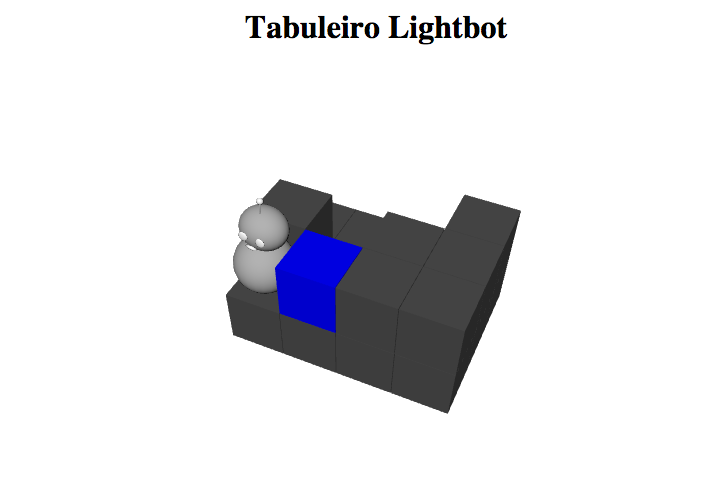
\includegraphics[scale=0.6]{tabuleiro1}
\\
Por fim, o \textit{keyValue} corresponde a todas as posições por onde o Robot tem que passar. A primeira posição do Robot é a posição inicial, depois fizemos uma função que calcula todas as posições por onde o Robot tem que passar, calculando as suas coordenadas.
Como não conseguimos desenvolver uma maneira eficiente, nem encontrar no \textit{X3DOM} uma maneira de mudar a cor do cubo enquanto o programa estivesse a correr, ou seja, num determinado tempo que iria corresponder ao tempo em que a lâmpada era acendida quando o comando L (Ligar Luz) o Robot fica na mesma posição e executa o comando seguinte.
\\
Contudo, tivemos ainda mais uma preocupação. O Robot só executa um comando se a posição seguinte for válida, ou seja, estiver dentro do tabuleiro. Isso foi feito através da seguinte função:\\

\begin{verbatim}
verifica :: Tab -> Pos -> Comandos -> Bool
verifica tab (x,y,o) c = if (x < (length (head tab))) && 
(x >=0) && (y < (length tab)) && (y>=0)
                            then True
                            else False
\end{verbatim}
\\
A avaliação no \textit{Mooshak} foi apenas qualitativa em que apenas verificava o output isto resultou numa avaliação aceite.

\section {Considerações Finais}

O projeto foi bastante útil e ajudou a desenvolver capacidades não só de programação como capacidades úteis no desenvolvimento de qualquer projeto de programação como, por exemplo a utilização de software para o controlo de versões como foi o caso do \textit{SVN}, a utilização de uma plataforma de avaliação automática do projeto como foi o caso do \textit{Mooshak} e software de edição do relatório, bastante útil em diversas componentes como foi o caso do \LaTeX.
Ficaram, no entanto, alguns problemas por resolver. Em primeiro lugar uma melhor estratégia para a resolução do Problema D que compreendesse a resolução de tabuleiros considerados mais difíceis e uma estratégia para mudar a cor de um cubo com lâmpada quando esta fosse acendida, relativamente ao Problema E.


\end {document}



